\documentclass[11pt]{article}
\usepackage[textwidth=18.0cm, textheight=23.0cm, top=2.0cm]{geometry}
\usepackage{pst-all}
\usepackage{amssymb}
\usepackage{tikz}
\usepackage{underscore}\begin{document}
\pagestyle{empty}


ClassName: \underline{\textbf{Class_08.2bp-4}}
\par
BinSize: \underline{\textbf{100 × 100}}
\par
ReduceSize: \underline{\textbf{100 × 100}}
\par
TypeNum: \underline{\textbf{20}}
\par
Num: \underline{\textbf{20}}
\par
OutS: \underline{\textbf{60000}}
\par
InS: \underline{\textbf{41715}}
\par
Rate: \underline{\textbf{0.695}}
\par
UB: \underline{\textbf{6}}
\par
LB0: \underline{\textbf{6}}
\par
LB: \underline{\textbf{6}}
\par
LBWithCut: \underline{\textbf{6}}
\par
NodeCut: \underline{\textbf{0}}
\par
ExtendedNodeCnt: \underline{\textbf{1}}
\par
GenNodeCnt: \underline{\textbf{1}}
\par
PrimalNode: \underline{\textbf{0}}
\par
ColumnCount: \underline{\textbf{6}}
\par
TotalCutCount: \underline{\textbf{0}}
\par
RootCutCount: \underline{\textbf{0}}
\par
LPSolverCnt: \underline{\textbf{1}}
\par
PricingSolverCnt: \underline{\textbf{0}}
\par
BranchAndBoundNum: \underline{\textbf{1}}
\par
isOpt: \underline{\textbf{true}}
\par
TimeOnPrimal: \underline{\textbf{0.000 s}}
\par
TimeOnPricing: \underline{\textbf{0.000 s}}
\par
TimeOnRmp: \underline{\textbf{0.069 s}}
\par
TotalTime: \underline{\textbf{0.130 s}}
\par
\newpage


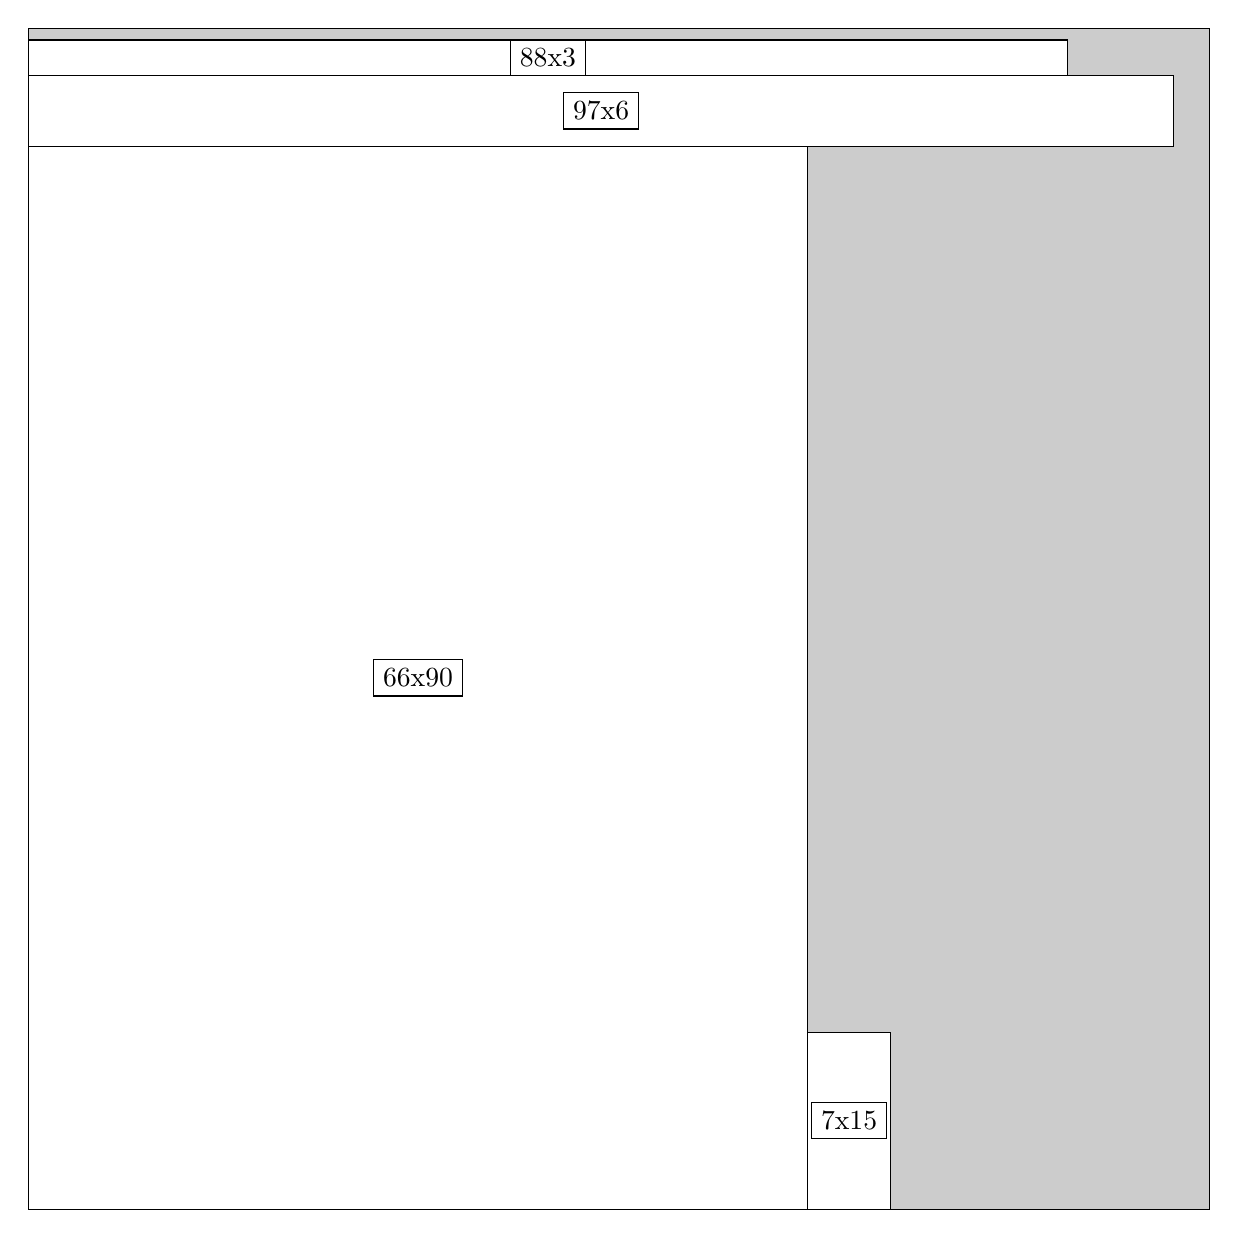
\begin{tikzpicture}[shorten >=1pt,scale=1.0,every node/.style={scale=1.0},->]
\tikzstyle{vertex}=[circle,fill=black!25,minimum size=14pt,inner sep=0pt]
\filldraw[fill=gray!40!white, draw=black] (0,0) rectangle (15.0,15.0);
\foreach \name/\x/\y/\w/\h in {66x90/0.0/0.0/9.9/13.5,97x6/0.0/13.5/14.549999999999999/0.8999999999999999,88x3/0.0/14.399999999999999/13.2/0.44999999999999996,7x15/9.9/0.0/1.05/2.25}
\filldraw[fill=white!40!white, draw=black] (\x,\y) rectangle node[draw] (\name) {\name} ++(\w,\h);
\end{tikzpicture}


w =66 , h =90 , x =0 , y =0 , v =5940
\par
w =97 , h =6 , x =0 , y =90 , v =582
\par
w =88 , h =3 , x =0 , y =96 , v =264
\par
w =7 , h =15 , x =66 , y =0 , v =105
\par
\newpage


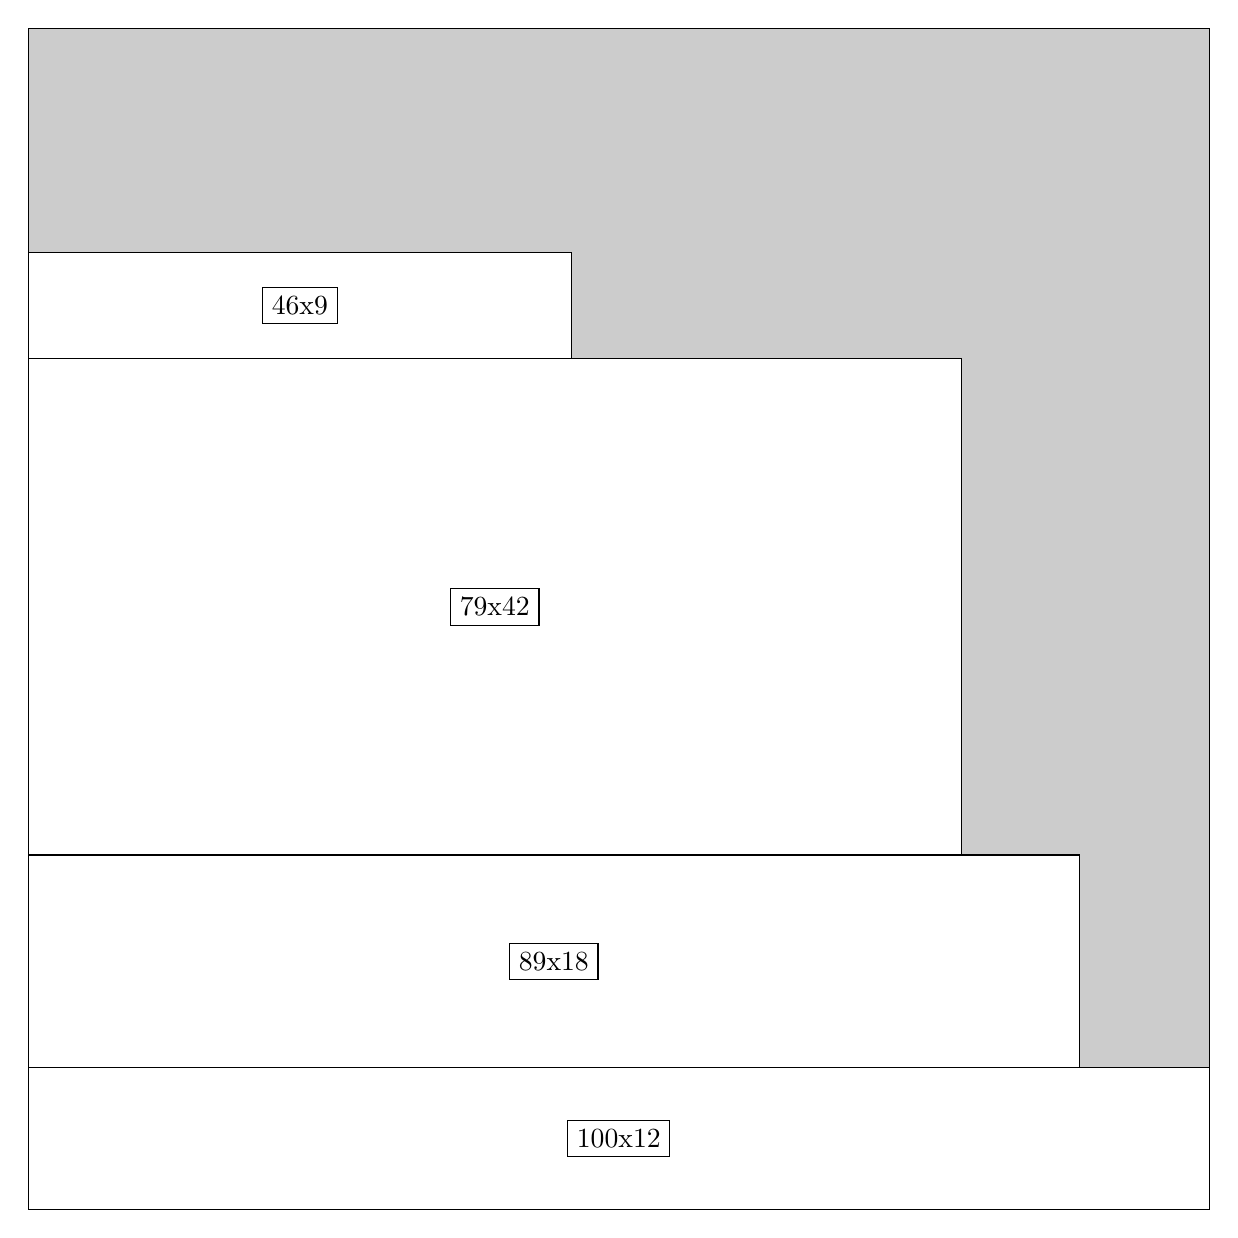
\begin{tikzpicture}[shorten >=1pt,scale=1.0,every node/.style={scale=1.0},->]
\tikzstyle{vertex}=[circle,fill=black!25,minimum size=14pt,inner sep=0pt]
\filldraw[fill=gray!40!white, draw=black] (0,0) rectangle (15.0,15.0);
\foreach \name/\x/\y/\w/\h in {79x42/0.0/4.5/11.85/6.3,89x18/0.0/1.7999999999999998/13.35/2.6999999999999997,100x12/0.0/0.0/15.0/1.7999999999999998,46x9/0.0/10.799999999999999/6.8999999999999995/1.3499999999999999}
\filldraw[fill=white!40!white, draw=black] (\x,\y) rectangle node[draw] (\name) {\name} ++(\w,\h);
\end{tikzpicture}


w =79 , h =42 , x =0 , y =30 , v =3318
\par
w =89 , h =18 , x =0 , y =12 , v =1602
\par
w =100 , h =12 , x =0 , y =0 , v =1200
\par
w =46 , h =9 , x =0 , y =72 , v =414
\par
\newpage


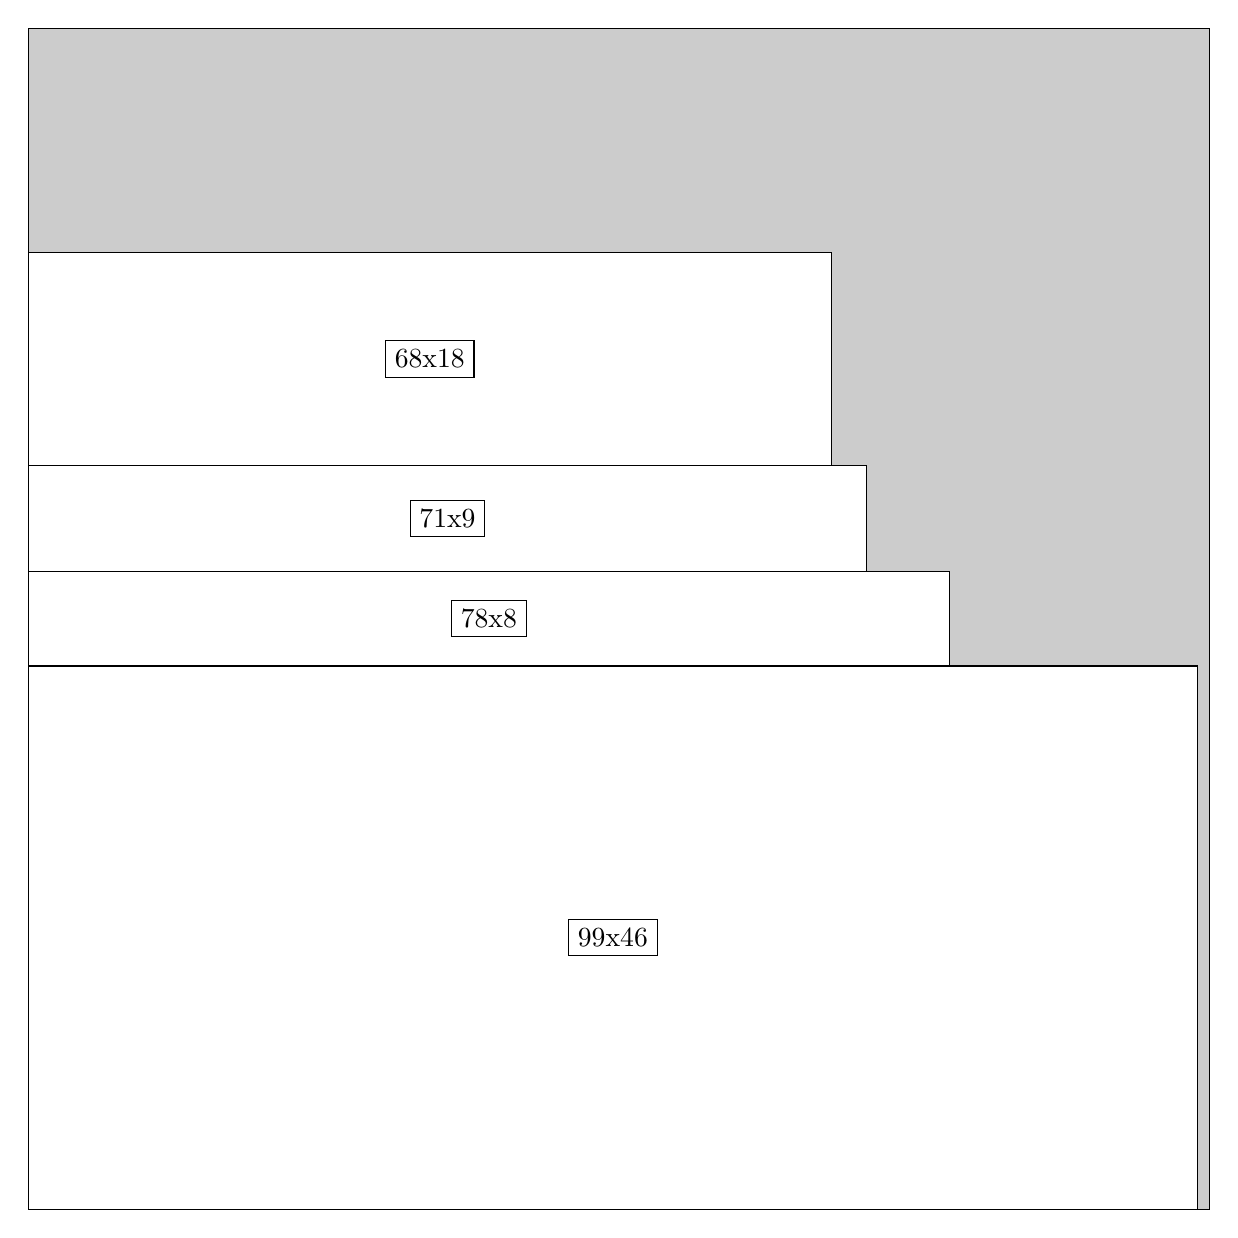
\begin{tikzpicture}[shorten >=1pt,scale=1.0,every node/.style={scale=1.0},->]
\tikzstyle{vertex}=[circle,fill=black!25,minimum size=14pt,inner sep=0pt]
\filldraw[fill=gray!40!white, draw=black] (0,0) rectangle (15.0,15.0);
\foreach \name/\x/\y/\w/\h in {99x46/0.0/0.0/14.85/6.8999999999999995,68x18/0.0/9.45/10.2/2.6999999999999997,71x9/0.0/8.1/10.65/1.3499999999999999,78x8/0.0/6.8999999999999995/11.7/1.2}
\filldraw[fill=white!40!white, draw=black] (\x,\y) rectangle node[draw] (\name) {\name} ++(\w,\h);
\end{tikzpicture}


w =99 , h =46 , x =0 , y =0 , v =4554
\par
w =68 , h =18 , x =0 , y =63 , v =1224
\par
w =71 , h =9 , x =0 , y =54 , v =639
\par
w =78 , h =8 , x =0 , y =46 , v =624
\par
\newpage


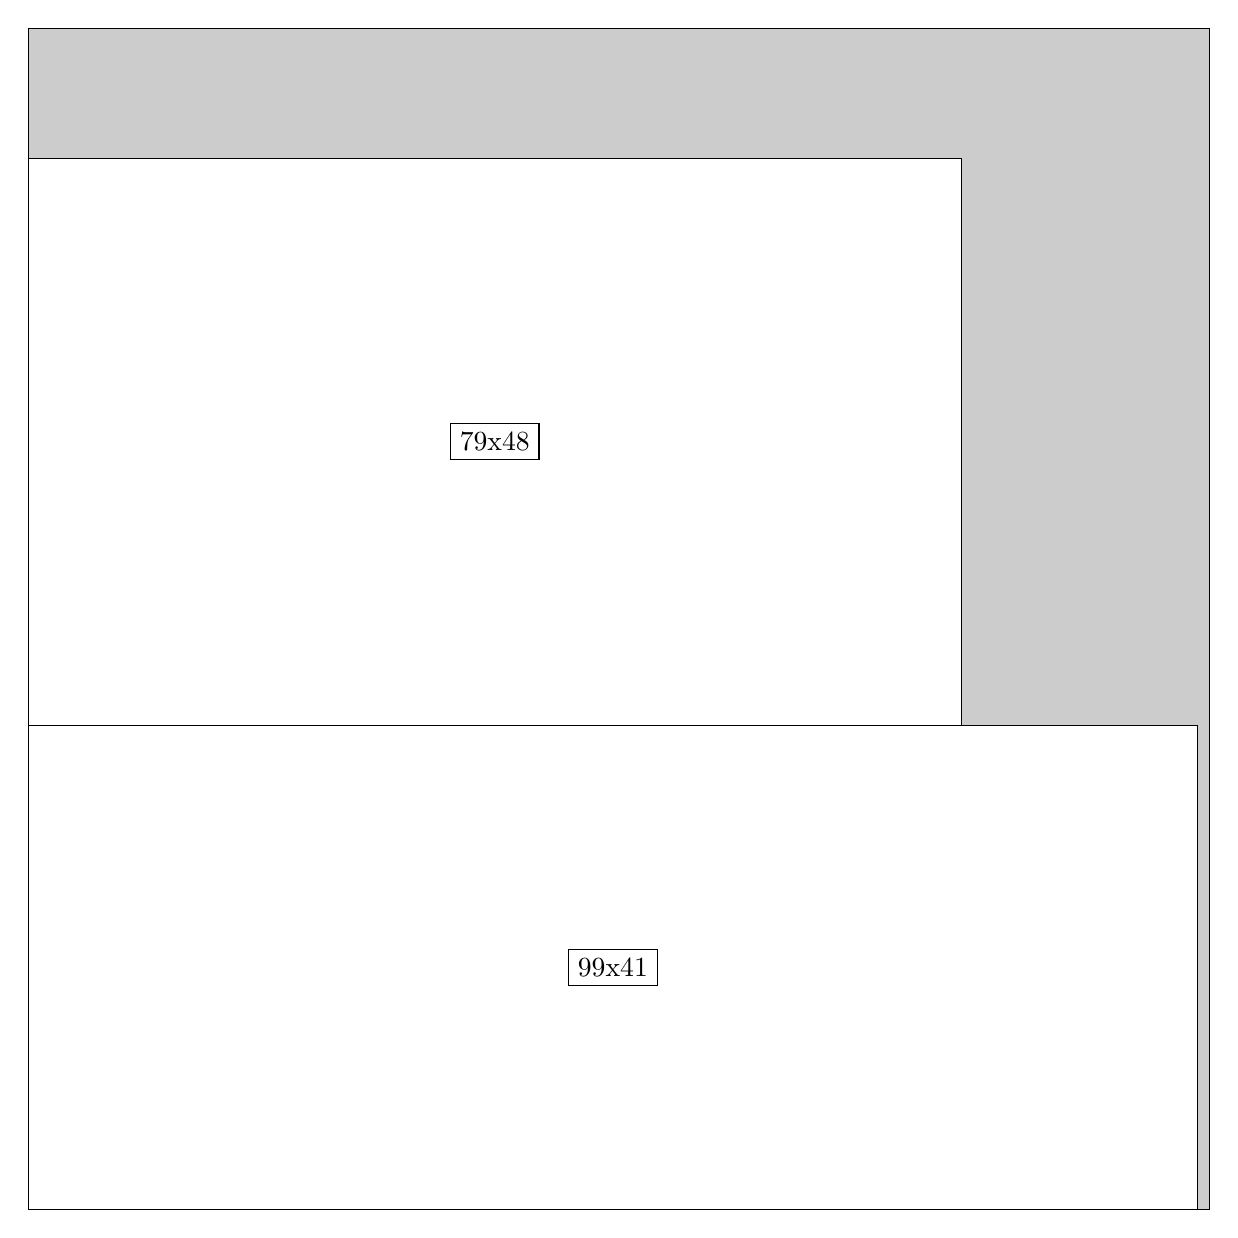
\begin{tikzpicture}[shorten >=1pt,scale=1.0,every node/.style={scale=1.0},->]
\tikzstyle{vertex}=[circle,fill=black!25,minimum size=14pt,inner sep=0pt]
\filldraw[fill=gray!40!white, draw=black] (0,0) rectangle (15.0,15.0);
\foreach \name/\x/\y/\w/\h in {99x41/0.0/0.0/14.85/6.1499999999999995,79x48/0.0/6.1499999999999995/11.85/7.199999999999999}
\filldraw[fill=white!40!white, draw=black] (\x,\y) rectangle node[draw] (\name) {\name} ++(\w,\h);
\end{tikzpicture}


w =99 , h =41 , x =0 , y =0 , v =4059
\par
w =79 , h =48 , x =0 , y =41 , v =3792
\par
\newpage


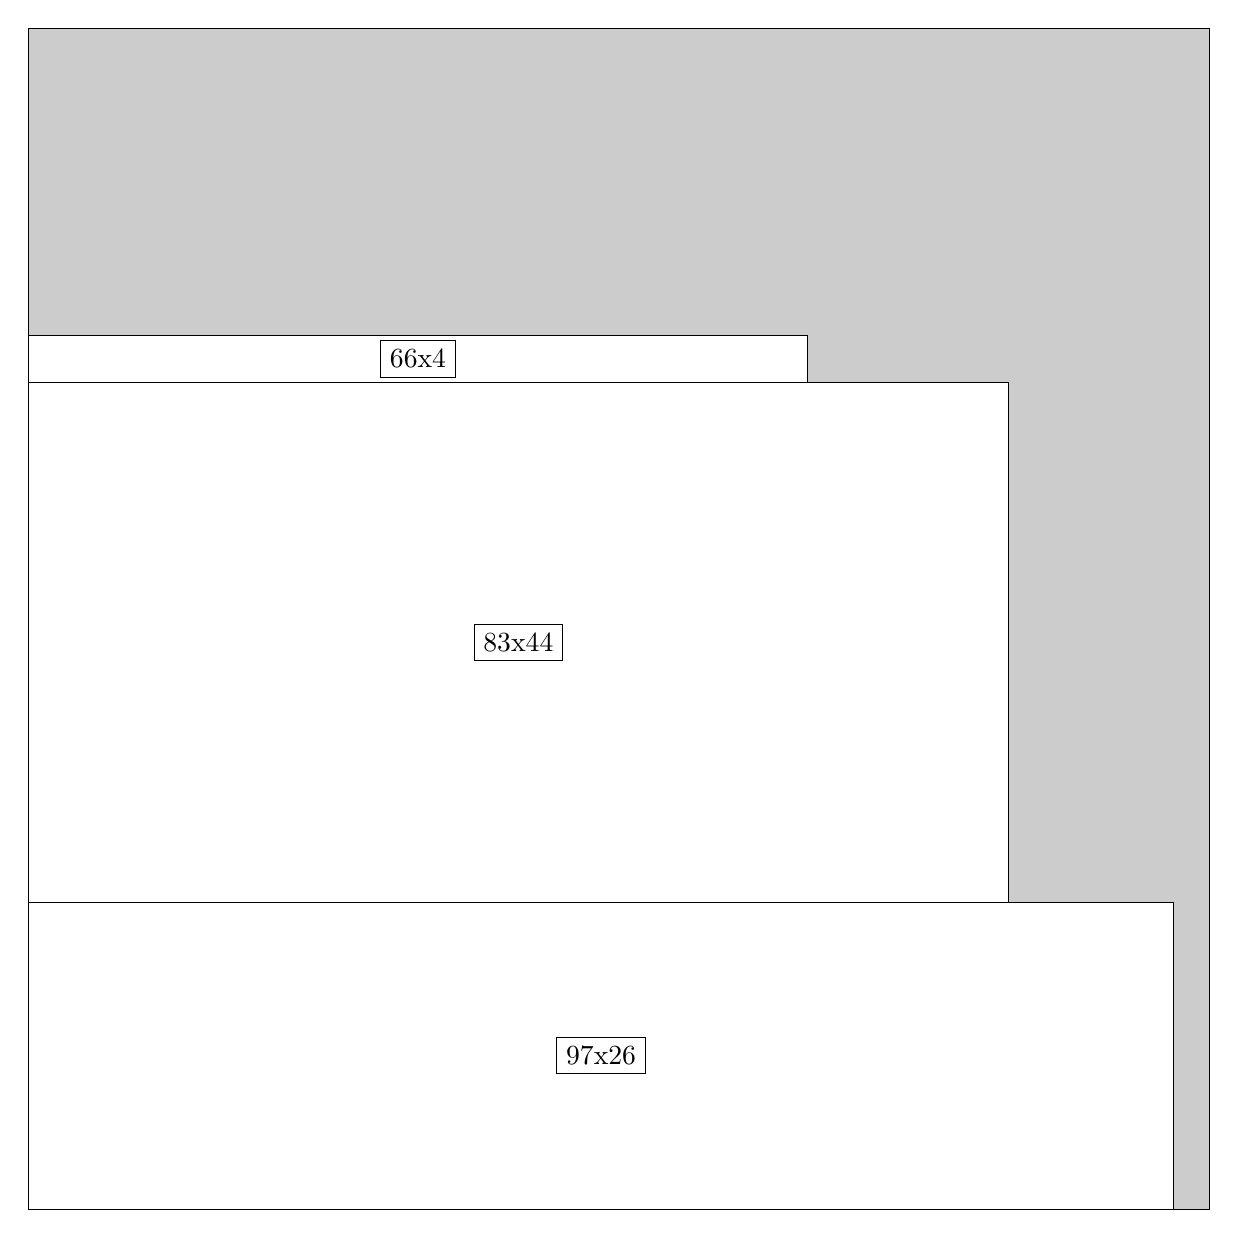
\begin{tikzpicture}[shorten >=1pt,scale=1.0,every node/.style={scale=1.0},->]
\tikzstyle{vertex}=[circle,fill=black!25,minimum size=14pt,inner sep=0pt]
\filldraw[fill=gray!40!white, draw=black] (0,0) rectangle (15.0,15.0);
\foreach \name/\x/\y/\w/\h in {83x44/0.0/3.9/12.45/6.6,97x26/0.0/0.0/14.549999999999999/3.9,66x4/0.0/10.5/9.9/0.6}
\filldraw[fill=white!40!white, draw=black] (\x,\y) rectangle node[draw] (\name) {\name} ++(\w,\h);
\end{tikzpicture}


w =83 , h =44 , x =0 , y =26 , v =3652
\par
w =97 , h =26 , x =0 , y =0 , v =2522
\par
w =66 , h =4 , x =0 , y =70 , v =264
\par
\newpage


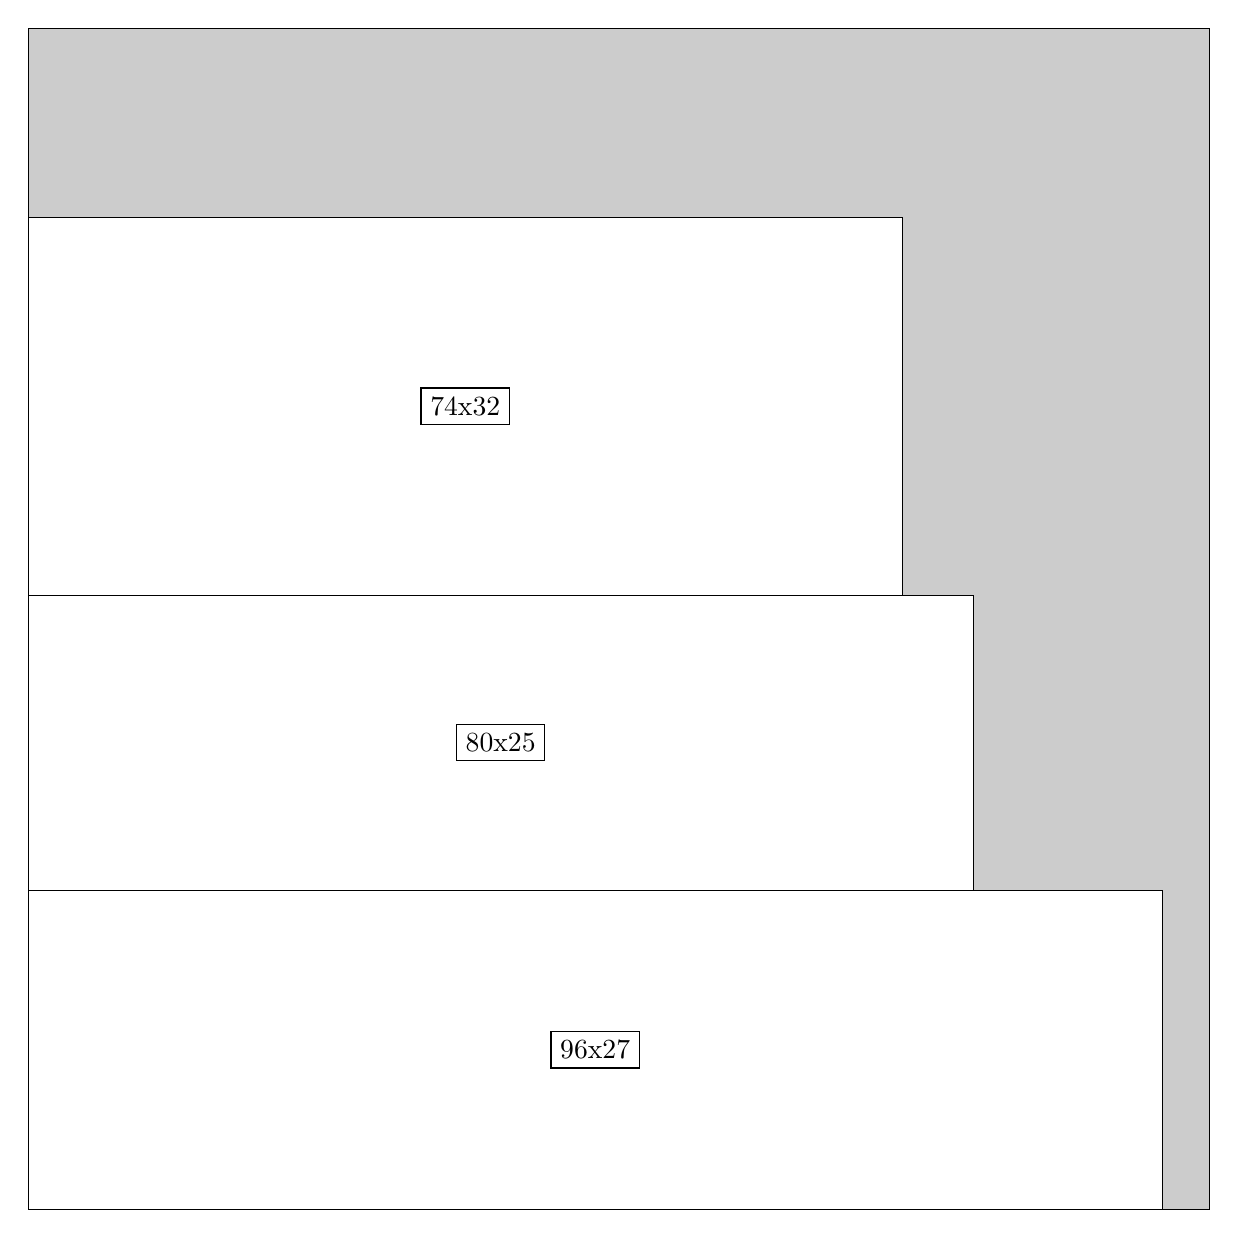
\begin{tikzpicture}[shorten >=1pt,scale=1.0,every node/.style={scale=1.0},->]
\tikzstyle{vertex}=[circle,fill=black!25,minimum size=14pt,inner sep=0pt]
\filldraw[fill=gray!40!white, draw=black] (0,0) rectangle (15.0,15.0);
\foreach \name/\x/\y/\w/\h in {96x27/0.0/0.0/14.399999999999999/4.05,74x32/0.0/7.8/11.1/4.8,80x25/0.0/4.05/12.0/3.75}
\filldraw[fill=white!40!white, draw=black] (\x,\y) rectangle node[draw] (\name) {\name} ++(\w,\h);
\end{tikzpicture}


w =96 , h =27 , x =0 , y =0 , v =2592
\par
w =74 , h =32 , x =0 , y =52 , v =2368
\par
w =80 , h =25 , x =0 , y =27 , v =2000
\par
\newpage


\end{document}